\begin{abstract}

As LLMs become capable of complex tasks, there is growing potential for personalized interactions tailored to the subtle and idiosyncratic preferences of the user.
We present a public benchmark, \textsf{PersonalLLM}, focusing on adapting LLMs to provide maximal benefits for a particular user. 
Departing from existing alignment benchmarks that implicitly assume uniform preferences, we curate open-ended prompts paired with many high-quality answers over which users would be expected to display heterogeneous latent preferences.
Instead of persona-prompting LLMs based on high-level attributes (e.g., user's race or response length), which yields homogeneous preferences relative to humans, we develop a method that can simulate a large user base with diverse preferences from a set of pre-trained reward models.
Our dataset and generated personalities offer an innovative testbed for developing personalization algorithms that grapple with continual data sparsity---few relevant feedback from the particular user---by leveraging historical data from other (similar) users.
We explore basic in-context learning and meta-learning baselines to illustrate the utility of \textsf{PersonalLLM} and highlight the need for future methodological development.
Our dataset is available at \url{https://huggingface.co/datasets/namkoong-lab/PersonalLLM}.

\end{abstract}


\section{Introduction}

The \textit{alignment} of LLMs with human preferences has recently 
received much attention, with a focus on adapting model outputs to reflect universal population-level values.
A typical goal is to take a pre-trained model that cannot reliably follow complex user instructions \citep{wei2022finetuned} and can easily be made to produce dangerous and offensive responses \citep{perez2022red} and adapt it to the instructions of its user base \citep{ouyang2022training} or train a generally helpful and harmless assistant \citep{bai2022training}. 
By assuming a \emph{uniform preference} across the population, recent successes~\citep{ziegler2020finetuning, ouyang2022training, christiano2023deep} demonstrate the feasibility of learning
and optimizing a monolithic preference (``reward model''). Alignment techniques have provided the basis for popular commercial applications like ChatGPT, as well as instruction-tuned open-source models \citep{touvron2023llama}.

The rapid advancement in LLM capabilities opens the door to an even more refined notion of human preference alignment: personalization.
A personalized model should adapt to the preferences and needs of a particular user, and provide maximal benefits as it accumulates interactions (see Figure~\ref{fig:main_figure}).
Given the expected data sparsity in this setting, beyond a particular user's data, such personalized language systems will likely also rely on historical data from other (similar) users in order to learn how to learn from a small set of new user feedback (see Figure~\ref{fig:metalearn}).
By discovering patterns across users, these systems will be able to efficiently optimize their responses, ultimately leading to more effective and beneficial conversational AI. 
We are motivated by the following potential use cases.
\begin{itemize}
\item Personalized learning experiences could be crafted by adapting educational chat assistants to the specific learning pace and style of individual students based on previous successful interactions with similar students.  
\item 
Customer support chatbots could offer more accurate and empathetic responses by drawing on a wealth of previous interactions, leading to quicker resolution times and higher customer satisfaction. 
\item In healthcare, personalized chatbots could provide tailored advice based on patients with similar medical histories and communication preferences. 
\end{itemize}

Compared to conventional applications where prompts have a uniform notion of ``ground truth'' (e.g., question answering),
LLM personalization is distinguished by the need to study open-ended prompts where users exhibit heterogeneous preferences across many possible high-quality answers (Figure~\ref{fig:main_figure}).
While personal preferences may vary according to simple features like user age \cite{chan2024scalingsyntheticdatacreation, castricato2024personareproducibletestbedpluralistic} and answer length and technicality \cite{li2024personalizedlanguagemodelingpersonalized}, they also involve more abstract dimensions of culture, politics, and language \cite{kirk2024prismalignmentprojectparticipatory}, as well as aspects of personality that are difficult to explain \citep{hwang2023aligninglanguagemodelsuser}.
A personalized LLM should be able to adapt to 
subtle, idiosyncratic, and sometimes sensitive differences between user tastes as it gathers more interactions.

\begin{figure}[t]
    \centering
    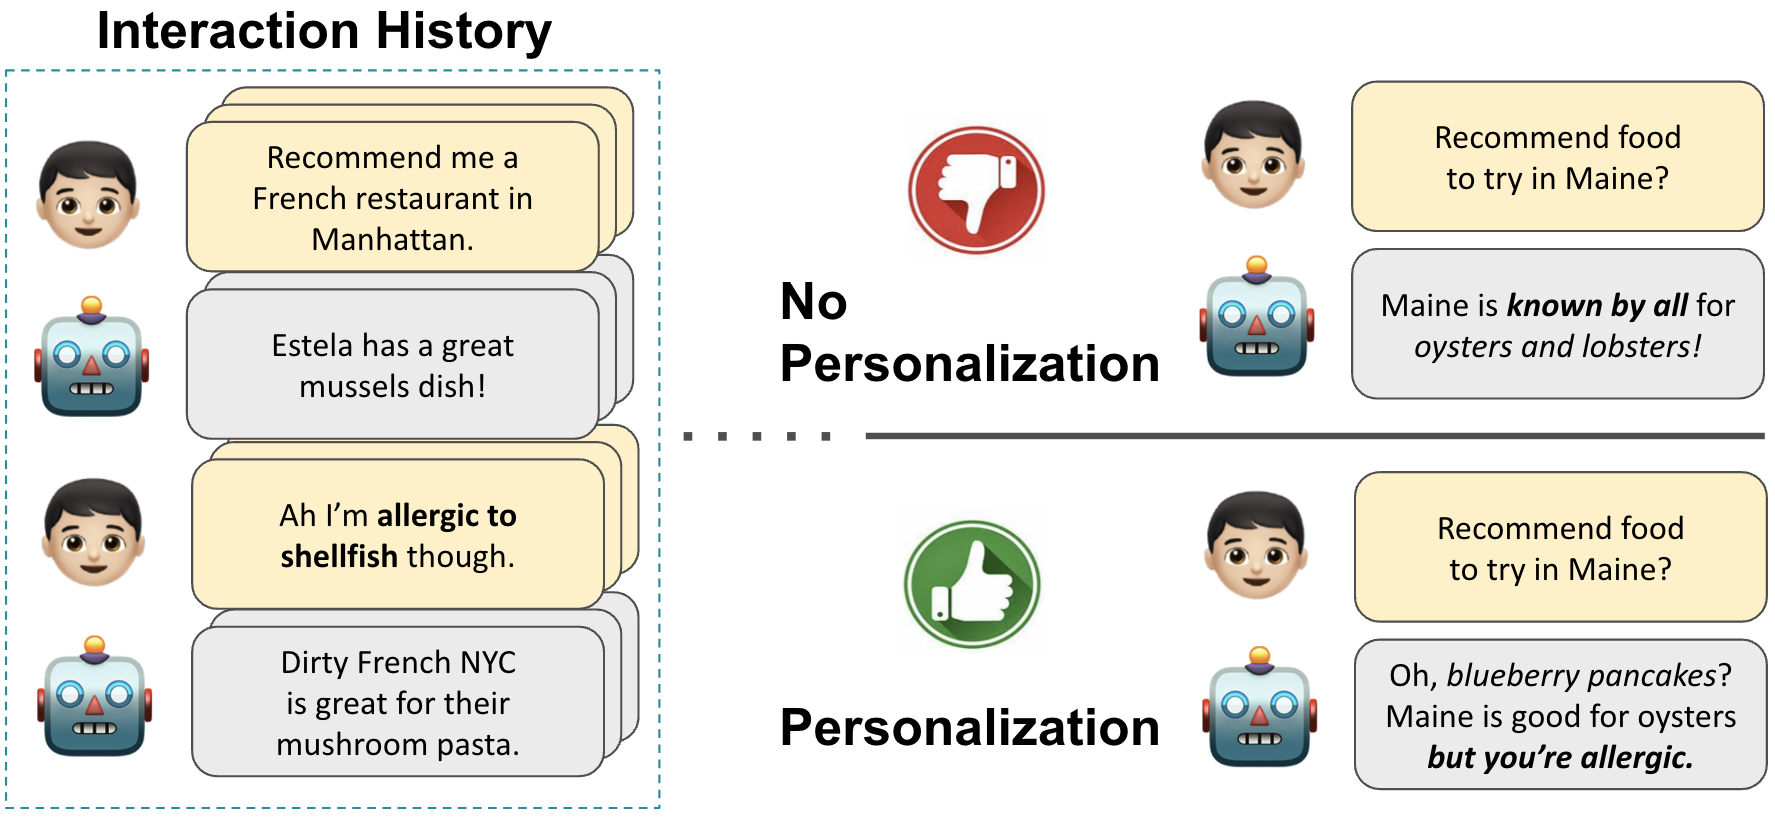
\includegraphics[width=\textwidth]{figures/fig1new.png}
    \caption{
    Standard LLMs require tedious re-prompting to learn a user’s preferences in each session. \textsf{PersonalLLM} aims to learn a unique user's diverse preferences to maximize long-term satisfaction.}
    \label{fig:main_figure}
\end{figure}

Inspired by the vision of a future with personalized AI, we introduce \textsf{PersonalLLM}, a public, open-source benchmark designed to adapt LLMs to provide maximal benefits for individual users. In order to explore complex differences in user tastes, our benchmark features a set of prompts with many high-quality LLM responses (from state-of-the-art LLMs like GPT-4o, Claude 3 Opus, and Gemini 1.5 Pro), such that humans \textit{are expected} to express diverse preferences over the responses.
Such an approach to dataset-building stands in contrast to existing alignment datasets, where responses exhibit observable quality differences (see Figure~\ref{fig:PersonalLLM}).

For each prompt and set of responses, our dataset also includes scores from a set of 10 reward models with heterogeneous preferences over those responses.
We leverage these reward models to sample many new ``users'' (or personal preference models) via weighted ensembles of their preferences, and in doing so we are able to \textit{simulate an entire user base}, which we argue to be a critical ingredient in a truly useful personalization benchmark.  
Through extensive analysis of the preferences of these users over our dataset, we show these simulated personal preference models to be diverse and non-trivial (e.g., with respect to length, formatting, or tone). We illustrate the difficulty of creating such an environment by comparing to the increasingly popular persona prompting baseline \citep{castricato2024personareproducibletestbedpluralistic, chan2024scalingsyntheticdatacreation, jang2023personalizedsoupspersonalizedlarge}, which in our analysis produces preferences only half as diverse as a set of \textsf{PersonalLLM} users across multiple metrics.
Taken together, the prompts, responses, and personalities present in \textsf{PersonalLLM} offer an innovative tested for benchmarking personalization algorithms as they tailor interactions based on previous interactions with an individual user.

While fine-tuning and reinforcement learning approaches \citep{schulman2017proximal, rafailov2023direct} are effective for aligning to population-level preferences,
personalization requires a new algorithmic toolkit, as it is not practical to gather enough data or
store a separate copy of the model or even low-rank adapter weights \citep{Hu2021} for every user.
\textsf{PersonalLLM} offers the versatility necessary to spur development across a range of new approaches to personalization: in-context learning (ICL) \citep{brown2020language}, retrieval augmented generation (RAG) \citep{lewis2021retrievalaugmented}, ranking agents, efficient fine-tuning, and other adaptation techniques.
In our experiments, we highlight a particularly salient challenge compared to typical applications of personalization in recommendation systems: the space of “actions/responses” is prohibitively large to be able to explore based on interactions on a single user. Since this necessitates  \textit{learning across users}, we model this as a meta-learning problem where the goal is to leverage a wealth of prior interactions from historical users to tailor responses for a new user who do not have a significant interaction history (see Figure~\ref{fig:metalearn}).

Motivated by key methodological gaps in personalizing LLMs, here we summarize our contributions:
\begin{itemize}
    \item  We release a new open-source dataset with over 10K open-ended prompts paired with 8 high-quality responses from top LLMs.
    \item We propose a novel method for sampling ``users'' (i.e., personal preference models) that, unlike existing methods, creates diverse preferences and allows for the simulation of large historical user bases.
    \item We illustrate new possibilities for algorithmic development in learning \textit{across} users.
\end{itemize}

Our goal in creating the open-source \textsf{PersonalLLM} testbed is to facilitate work on methods to personalize the output of an LLM to the individual tastes of many diverse users.
We do not claim our simulated personal preference models provide a high-fidelity depiction of human behavior, but rather offer a challenging simulation environment that provides the empirical foundation for methodological innovation in capturing the complex array of human preferences that arise in practice.
As an analogy, while ImageNet \citep{russakovsky2015imagenetlargescalevisual} is noisy and synthetic---e.g., differentiating between 120 dog breeds is not a realistic vision task---it provides a challenging enough setting that methodological progress on ImageNet implies progress on real applications.
Similarly, we believe \textsf{PersonalLLM} is a reasonable initial step toward the personalization of language-based agents, building on the common reinforcement learning paradigm of benchmarking personalization algorithms with simulated rewards \citep{zhao2023kuaisimcomprehensivesimulatorrecommender, ie2019recsimconfigurablesimulationplatform}.

